\documentclass[crop,tikz,border=10px,convert=pdf2svg,multi=false]{standalone}
\usepackage[defaultsans]{opensans}
\usetikzlibrary{shapes,arrows,positioning}
\begin{document}
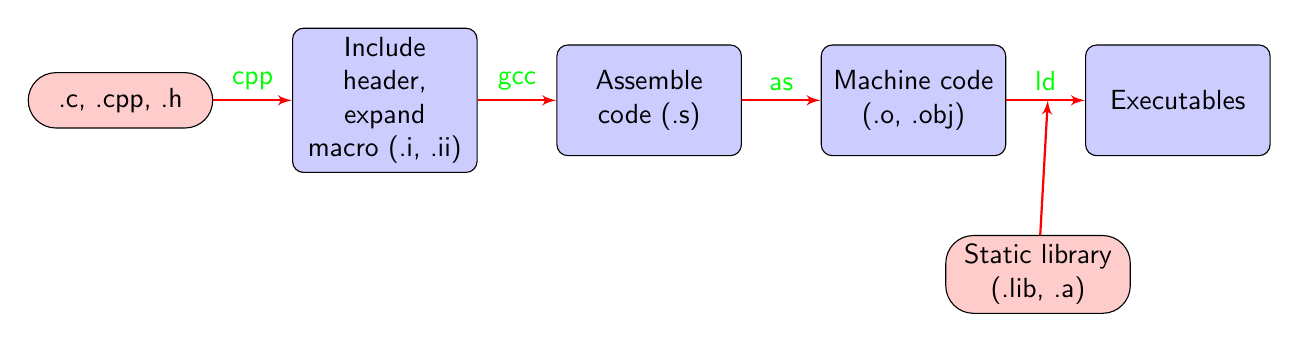
\begin{tikzpicture}[font=\sffamily,remember picture,
  block/.style = {rectangle, draw, fill=blue!20, text centered, text
    width=6em, rounded corners, minimum height=4em},
  cloud/.style = {rectangle, draw, fill=red!20, text centered, text
    width=6em, rounded corners=10pt, minimum height=2em},
  line/.style = {-latex', red, thick},
  linetext/.style = {green, midway,text centered, above},
  title/.style = {draw=none, font=\Large\bf\sffamily, text centered}]

  \node [cloud] (src) {.c, .cpp, .h};
  \node [block, right=of src] (pp) {Include header, expand macro (.i, .ii)};
  \node [block, right=of pp] (compiler) {Assemble code (.s)};
  \node [block, right=of compiler] (assembler) {Machine code (.o, .obj)};
  \node [block, right=of assembler] (linker) {Executables};

  \node [cloud, below=of assembler,xshift=4.5em] (static) {Static library (.lib, .a)};

  \draw [line] (src) -- (pp) node[linetext] () {cpp};
  \draw [line] (pp) -- (compiler) node[linetext] () {gcc};
  \draw [line] (compiler) -- (assembler) node[linetext] () {as};
  \draw [line] (assembler) -- (linker) node[linetext] () {ld};

  \coordinate [right=1.5em of assembler] (tmp);
  \draw [line] (static) -- (tmp);

\end{tikzpicture}
\end{document}
